\documentclass[11pt]{article}

% font
\usepackage{tgschola}
\usepackage{amsmath}

\usepackage{graphicx}
\usepackage{subfig}
\usepackage{float}
\usepackage[T1]{fontenc}
\usepackage[utf8]{inputenc}
\usepackage[english]{babel}
\usepackage{multicol}
\usepackage[ddmmyyyy]{datetime}
\usepackage[a4paper, margin=2cm]{geometry}

% sections on new page
\usepackage{titlesec}
\newcommand{\sectionbreak}{\clearpage}
\setcounter{secnumdepth}{0}

% index and clickable toc
\usepackage{hyperref}
\hypersetup{
	colorlinks,
	citecolor=black,
	filecolor=black,
	linkcolor=black,
	urlcolor=black
}

% bibliography
\usepackage[
	%backend=biber,
	style=numeric,
	citestyle=ieee
]{biblatex}
\usepackage{csquotes}

\addbibresource{bibliography.bib}

% table of content name
\addto\captionsenglish{% Replace "english" with the language you use
	\renewcommand{\contentsname}%
	{\hfill \Huge Table of Content \hfill}%
}

\begin{document}

	% Title page
	\begin{titlepage}
		\begin{center}

			\vspace*{0.5cm}

			% title
			\Huge
			\textbf{Brain Tumor Detection}

			\vspace{0.8cm}

			% logo
			
\includegraphics[width=0.4\linewidth]{imgs/cu_logo.png}

			\vspace{1cm}

			\normalsize
			Department of Computer Science\\
			Gurudas College\\
			Calcutta University\\
			\today

			% subtitle
			\vspace{0.5cm}
			\textit{Detection of tumorous cells using machine learning models}

			\vspace{1cm}

			\normalsize
			Submitted in partial fulfillment for the requirements for the
			degree Bachelor of Science (Honors) in Computer Science.

			Academic Year: \textbf{2018-2021}

			\vfill
			% author
			\textbf{Authors}:

			$\bullet$ Shoptorshi \space\space
			$\bullet$ Brahmajit \space\space
			$\bullet$ Rajarshi \space\space
			$\bullet$ Bhargav

			% supervisor
			\vspace{1cm}
			\rule{5cm}{0.4pt}

			\textbf{Supervisor}: Kajari Bhattacharjeee

		\end{center}
	\end{titlepage}

	% certificate page
	\section[certificate]{\hfill \Huge Certificate \hfill}
	%\thispagestyle{empty}

	% roman page numbering
	\pagenumbering{roman}

	\begin{center}
		\vspace{1cm}

		% logo
		
\includegraphics[width=0.3\linewidth]{imgs/cu_logo.png}

		\vspace{1cm}

		\Large
		Department of Computer Science\\
		Gurudas College\\
		Calcutta University\\
	\end{center}

	\vspace{1.8cm}
	This is to certify that the project entitled "Brain tumor detection using
	Machine Learning models" is a bona fide work of \textbf{Shoptorshi},
	\textbf{Brahmajit}, \textbf{Rajarshi} and \textbf{Bhargav} submitted to
	Gurudas College, University of Calcutta; in partial fulfillment of the
	requirement for the award of the degree "Bachelor of Science (Honors)" in
	Computer Science.
	\vfill

	\begin{multicols}{2}

		Supervisor:

		\rule{5cm}{0.4pt}

		\textbf{Kajari Bhattacharjeee}

		\vspace{1cm}

		Department

		Head:

		\rule{5cm}{0.4pt}

		\textbf{Srijeeta Charkraborty}


		\columnbreak

		Principal:

		\rule{5cm}{0.4pt}

		\textbf{Dr. Mausumi Chatterjee}

	\end{multicols}

	\section[acknowledgement]{\hfill \Huge Acknowledgement \hfill}
	\label{sec:Acknowledgement}

	\vspace{1cm}

	I would like to express my special thanks of gratitude to our supervisor
	\textbf{Kajari Bhattacharjeee}, teachers of our department \textbf{Sonali
	Gupta} and \textbf{Srijeeta Charkraborty} ( current department head ); as
	well as our principal ma'am \textbf{Dr. Mausumi Chatterjee} who gave us the
	golden opportunity to do this wonderful project on \textit{Brain tumor
	detection}, which has also helped us in doing a lot of research and we came
	to know about many new things.

	We are really thankful to them.

	\vspace{1cm}

	Secondly we would like to thank the incredible authors of the research
	papers in our references/citations for providing us with the information.

	\tableofcontents

	% abstract
	\section[abstract]{}

	% reverting back to normal page numbering
	\pagenumbering{arabic}

	\thispagestyle{plain}
	\begin{center}
		\Large
		\textbf{Brain Tumor Detection}

		\vspace{0.4cm}
		\large
		Using various machine learning models to detect brain tumor.

		\vspace{0.5cm}
		\textbf{Abstract}
	\end{center}

	Tumors are cancerous or non-cancerous mass or growth of abnormal cells in
	brain. Tumors can start in brain, or cancer elsewhere in the body can spread
	to brain. There are many way to control the occurrence of these abnormal
	cells. A tumor can be denoted as a malformed mass of tissues wherein the
	cells multiply abruptly and ceaselessly, that is there is no control over
	the growth of the cells.

	The process of Image segmentation is adopted for extracting abnormal tumor
	region within the brain. In the MRI (magnetic resonance image), segmentation
	of brain tissue holds very significant in order to identify the presence of
	outlines concerning the brain tumor. There is abundance of hidden
	information in stored in the Health care sector. With appropriate use of
	accurate data mining classification techniques, early prediction of any
	disease can be effectively performed.

	The project examines list of risk factors that are being traced out in brain
	tumor surveillance systems. Also the method proposed assures to be highly
	efficient and precise for brain tumor detection, classification and
	segmentation. To achieve this precise automatic or semi-automatic methods
	are needed. The project proposes an automatic segmentation method that
	relies upon \textit{ CNN (Convolution Neural Networks) }, \textit{ VGG 16 }
	and \textit{ Resent 50 }, determining small 7 x 7 kernels. By incorporating
	this single technique, segmentation and classification is accomplished. CNN
	(a ML technique) from NN (Neural Networks)wherein it has layer based for
	results classification.

	Various levels involved in the proposed mechanisms are:

	\begin{enumerate}
		\item \textbf{ Data collection }
		\item \textbf{ Pre-processing }
		\item \textbf{ Average filtering }
		\item \textbf{ segmentation }
		\item \textbf{ feature extraction }
		\item \textbf{CNN (or any other model) via classification and identification. By
			utilizing the DM (data mining) techniques, significant relations and
			patterns from the data can be extracted. The techniques of ML
			(machine learning) and Data mining are being effectively employed
			for brain tumor detection and prevention at an early stage.}
	\end{enumerate}

	\section[introduction]{\hfill \Huge Introduction \hfill}
	\subsection[domain description]{Domain Description}

	\begin{enumerate}
		\item \textbf{Neurological Examination}: It is a series of test to
			measures the function of the patients nervous system and also
			his/her physical and mental alertness.
		\item \textbf{Machine Learning}: Machine learning approaches address
			these problems by mainly using hand-crafted features (or pre-defined
			features). As an initial step in this kind of segmentation, the key
			information is extracted from the input image using some feature
			extraction algorithm, and then a discriminative model is trained to
			recognize the tumor from normal tissues. The designed machine
			learning techniques generally employ hand-crafted features with
			various classifiers, such as random forest, support vector machine
			(SVM), fuzzy clustering. The designed methods and features
			extraction algorithms have to extract features, edge-related
			details, and other necessary information—which is time-consuming.
			Moreover, when boundaries between healthy tissues and tumors are
			fuzzy/vague, these methods demonstrate poorer performances.
		\item \textbf{Brain Scan}: Brain scan is a picture of the internal
			structure of the brain. A specialized machine takes a scan in the
			same way as a digital camera takes a photograph. Using computer
			technology, a scan compiles an image of the brain by photographing
			it from various angles. Some types of scan uses contrast agent (or
			contrast dye), which helps the doctor to see the difference between
			normal and abnormal brain tissues.

			MRI (Magnetic Resonance Imaging): It is a scanning device that uses
			magnetic field and computer to capture images of the brain on films.
			It does not use x-rays. It provides pictures from various planes,
			which permits doctor to create a three-dimensional image of the
			tumor. The MRI detects signals emitted from normal and abnormal
			tissues, providing clear images of almost all tumors.
	\end{enumerate}

	\subsection[motivation]{Motivation}
	The motivation is to develop a software with better segmentation capability
	for use in medical imaging to detect diseases like brain tumor. Image
	segmentation has been identified as the key problem of medical image
	analysis and remains a popular and challenging area of research. Image
	segmentation is increasingly used in many clinical and research applications
	to analyze medical imaging datasets; which motivated us to present a
	snapshot of dynamically changing field of medical image segmentation.

	CT (Computed Tomography), MRI (Magnetic Resonance Imaging), PET (Positron
	Emission Tomography) etc. generates a large amount of image information.
	With the improved technology, not only does the size and resolution of the
	images grow but also the number of dimensions increases. In the future, we
	would like to have algorithms which can automatically detect diseases,
	lesions and tumors, and highlight their locations in the large pile of
	images.

	The motivation of this work is to increase patient safety by providing
	better and more precise data for medical decision.

	\subsection[scope of work]{Scope of Work}
	\subsubsection[deliverables]{Deliverables}
	\begin{itemize}
		\item Working program to take an MRI scan as input and predict presence
			of tumorous cells with $\geq 90\%$ accuracy.
	\end{itemize}

	\subsubsection[scope]{Scope}
	\begin{itemize}
		\item The working program has external dependencies ( libraries ) and
			it's expected to have a them installed for the program to work.
	\end{itemize}

	\subsubsection[timeline]{Timeline}
	\begin{itemize}
		\item \textbf{April 27, 2021} Project Assigned
		\item \textbf{May 2, 2021} Project finalized by supervisor, and group is
			divided into groups of two.
		\item \textbf{May 3, 2021} Data collection started.
		\item \textbf{May 12, 2021} Project Repository created and coding is
			started.
		\item \textbf{July 7, 2021} Coding is finished, documentation is
			started.
		\item \textbf{Just 21, 2021} Documentation complete.
	\end{itemize}

	\subsubsection[reports]{Reports}
	\begin{itemize}
		\item Constantly updating and pushing code to repository.
		\item Both teams staying in touch with each other to keep up with each
			others progress.
		\item Report back to supervisor every once a week.
	\end{itemize}

	\section[background]{\hfill \Huge Background \hfill}

	Natarajan \cite{bac1} proposed brain tumor detection method for MRI brain
	images. The MRI brain images are first preprocessed using median filter,
	then segmentation of image is done using threshold segmentation and
	morphological operations are applied and then finally, the tumor region is
	obtained using image subtraction technique. This approach gives the exact
	shape of tumor in MRI brain image. Joshi \cite{bac2}  proposed brain tumor
	detection and classification system in MR images by first extracting the
	tumor portion from brain image, then extracting the texture features of the
	detected tumor using Gray Level Co- occurrence Matrix (GLCM) and then
	classified using neuro-fuzzy classifier. Amin and Mageed \cite{bac3}
	proposed neural network and segmentation base system to automatically detect
	the tumor in brain MRI images. The Principal Component Analysis (PCA) is
	used for feature extraction and then Multi-Layer Perceptron (MLP) is used
	classify the extracted features of MRI brain image.  The average recognition
	rate is 88.2\% and peak recognition rate is 96.7\%.  Sapra \cite{bac4}
	proposed image segmentation technique to detect brain tumor from MRI images
	and then Probabilistic Neural Network (PNN)  is used for automated brain
	tumor classification in MRI scans. PNN system proposed handle the process of
	brain tumor classification more accurately. Suchita and Lalit \cite{bac5}
	proposed unsupervised neural network learning technique for classification
	of brain MRI images.  The MRI brain images are first preprocessed which
	include noise filtering, edge detection, then the tumor is extracted using
	segmentation. The texture features are extracted using Gray-Level
	Co-occurrence Matrix(GLCM) and then Self-Organizing Maps (SOM) are used to
	classify the brain as normal or abnormal brain, that is, whether it contain
	tumor or not. Rajeshwari and Sharmila \cite{bac6} proposed preprocessing
	techniques which are used to improve the quality of MRI image before using
	it into an application. The average, median and wiener filters are used for
	noise removal and interpolation based Discrete Wavelet Transform (DWT)
	technique is used for resolution enhancement. The Peak Signal to Noise Ratio
	(PSNR) is used for evaluation of these techniques.

	\section[methodology]{\hfill \Huge Methodology \hfill}

	As per literature survey, it was found that automated  brain  tumor
	detection  is  very  necessary  as  high accuracy is needed when human life
	is involved.  Automated detection of tumor in MR images involves feature
	extraction and  classification  using  machine  learning  algorithm.  In
	this paper, a system to automatically detect tumor in MR images is proposed
	as shown in Figure~\ref{Proposed Methodology}

	\begin{figure}[h]
		\centering
		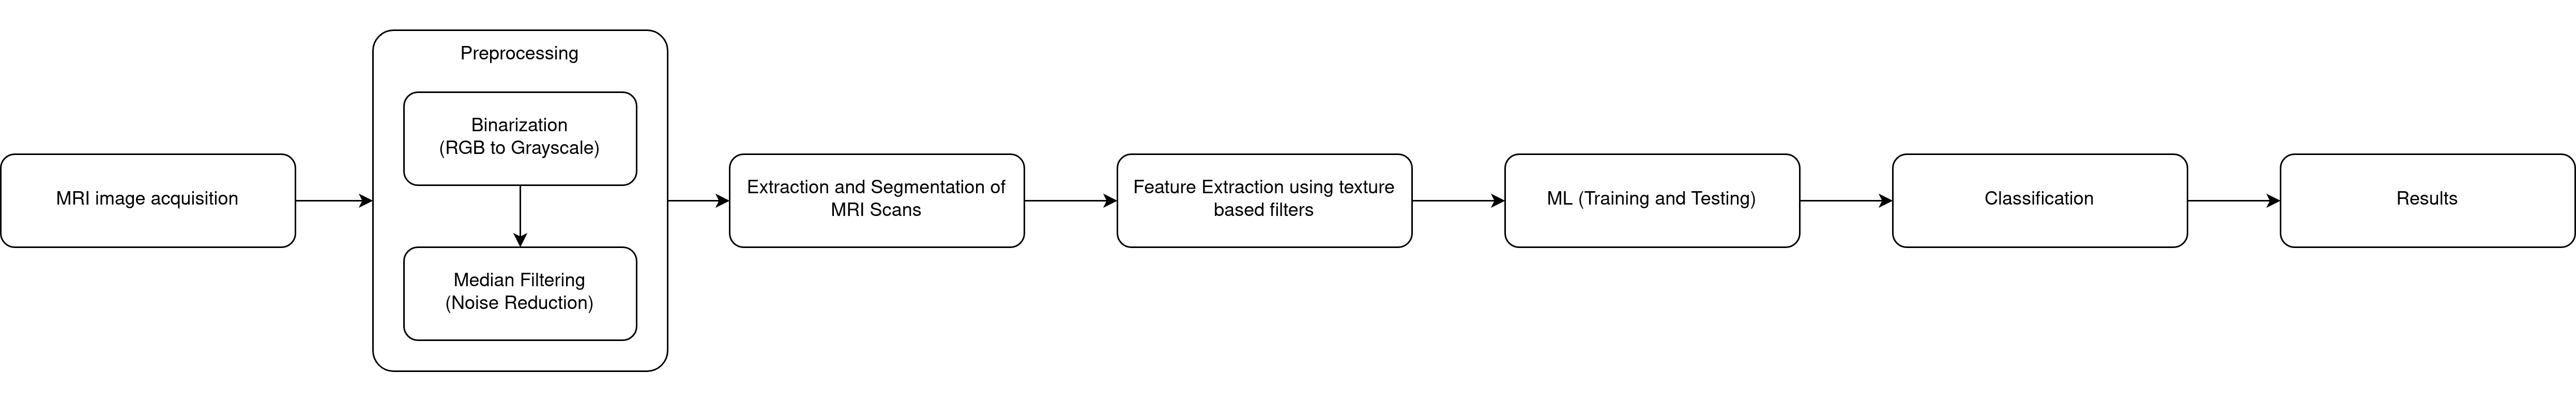
\includegraphics[width=1\linewidth]{imgs/methodology}
		\caption{Proposed Methodology}%
		\label{Proposed Methodology}
	\end{figure}

	\subsection{Image Acquisition}%
	\label{sub:Image Acquisition}

	The MRI brain images are acquired and are
	given as input to pre-processing stage. The sample brain MR images are shown
	in Figure~\ref{MRIScans}.

	\begin{figure}[H]
		\centering
		\subfloat[MRI scan shown no presence of tumor]
		{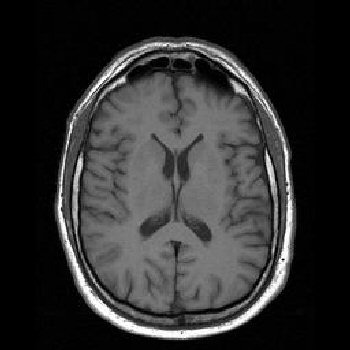
\includegraphics[width=0.4\linewidth]
		{imgs/pred1.jpg}\label{scan2}}
		\hspace{0.5cm}
		\subfloat[MRI scan of a tumorous cell]
		{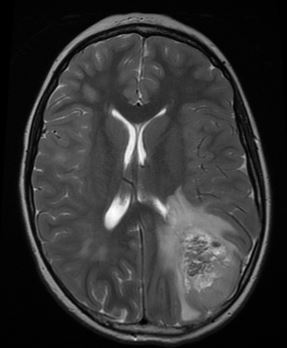
\includegraphics[width=0.3\linewidth]
		{imgs/Y100.JPG}\label{scan1}}
		\caption{MRI Scans}
		\label{MRIScans}
	\end{figure}

	\subsection{Preprocessing}%
	\label{sub:Preprocessing}

	Preprocessing is needed as it provides improvement
	in image data which  enhances some of the image features which are important
	for further processing. The  pre-processing steps that are applied to MR
	image are as follows:

	\begin{enumerate}
		\item The  RGB  MR    image  is  converted  to  gray  scale image  and
			then  median  filter  is  applied  for  noise  removal from brain MR
			images as shown in Figure~\ref{smooted image}. The noise is to removed for further
			processing as high accuracy is needed.

		\item Then  edges  are  detected  from  filtered  image  using canny
			edge  detection  as  shown  in  Figure~\ref{edge detection}.  The  edge detected
			image is needed for segmentation of  the image

		\item Then  watershed  segmentation  is  done  for  finding the
			location  of  the  tumor  in  the  brain  image  as  shown  in
			Figure~\ref{segmentation}. Segmentation is  the process of dividing  an image into
			multiple segments. The aim of segmentation is to change
			representation  of    image  into  something  which  is more  easy
			to  analyze.  The result  of  watershed  segmentation is  label
			image.    In  label  image,  all  the  different  objects identified
			will  have  different  pixel  values  ,  all  the  pixels  of first
			object  will have value 1, all the pixels of second object will have
			value 2 and so on.
	\end{enumerate}


	\begin{figure}[H]
		\centering
		\subfloat[Original Image]
		{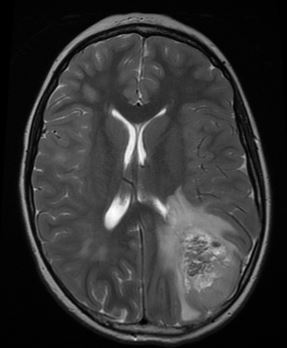
\includegraphics[width=0.2\linewidth]
		{imgs/Y100.JPG}\label{original}}
		\hspace{0.5cm}
		\subfloat[Filtered Imaage]
		{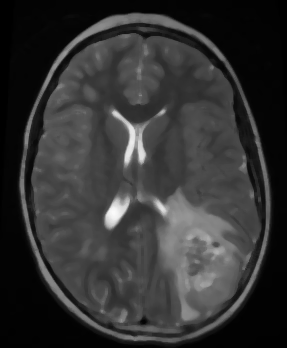
\includegraphics[width=0.2\linewidth]
		{imgs/median_filtering.png}\label{smooted image}}
		\hspace{0.5cm}
		\subfloat[Edge Detection]
		{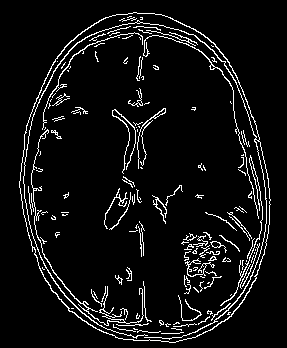
\includegraphics[width=0.2\linewidth]
		{imgs/edges_detection.png}\label{edge detection}}
		\hspace{0.5cm}
		\subfloat[Segmentation]
		{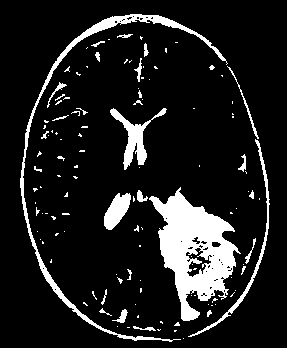
\includegraphics[width=0.2\linewidth]
		{imgs/segmentation.png}\label{segmentation}}
		\caption{preprocessing operations}
		\label{Preprocessing Operations}
	\end{figure}

	\subsection{Feature Extraction}%
	\label{sub:Feature Extraction}

	When input to an algorithm is very large and
	redundant to be processed, it is transformed into reduced representative set
	of features called feature vector. Transformation of input data into set of
	features is called feature extraction. In this step, the important features
	needed for image classification are extracted. The segmented brain MR image
	is used and texture features are extracted from the segmented image which
	shows the texture property of the image. These features are extracted using
	Gray Level Co-occurrence Matrix (GLCM) as it is robust method with high
	performance.

	The GLCM features are extracted as follows:

	\begin{enumerate}
		\item Energy: It gives a measure of textural uniformity, that is, measure
			of pixel pair repetitions.

			\begin{equation}
				E = \sum^{N_g - 1}_{i=0} \sum^{N_g - 1}_{j=0} p(i, j)^2 \
				\textnormal{ here, range = [0,1] }
			\end{equation}

		\item Contrast: It gives a measure of intensity contrast between a pixel
			and its neighbor over the whole image.

			\begin{equation}
				Con = \sum^{N_g -1}_{n=0} n^2 \sum^{N_g -1}_{i=0} \sum^{N_g
				-1}_{j=0} p(i,j)^2 \
				\textnormal{ here, range = [0,1] }
			\end{equation}

		\item Correlation: It gives a measure of how correlated a pixel to its
			neighbor over the whole image.

			\begin{equation}
				C = \frac{1}{\sigma^x \sigma^y}
				\sum^{N_g - 1}_{i=0} \sum^{N_g -1}_{j=0} (i,j) p(i,j)^2
				- \mu_x \mu_y \ \textnormal{here, range = [-1,1]}
			\end{equation}

		\item Homogeneity: It gives a measure of closeness of distribution of
			elements in GLCM to GLCM diagonal.

			\begin{equation}
				H = \sum^{N_g -1}_{i=0} \sum^{N_g -1}_{j=0}
				\frac{p(i,j)}{1 + \pmod{i,j}}
				\ \textnormal{here, range = [0, 1]}
			\end{equation}
	\end{enumerate}

	\subsection{Classification}%
	\label{sub:Classification}

	The Machine learning algorithms are used for
	classification of MR brain image either as normal or abnormal.  The major
	aim of ML algorithms is to automatically learn and make intelligent
	decisions. The feature set formed by above specified method was applied to
	Multi-Layer Perceptron (MLP) and Naive Bayes for classification.  MLP [3] is
	a feed forward artificial neural network model that maps sets of input data
	into a set of appropriate output. It is known as feed forward because it
	does not contain any cycles and network output depends only on the current
	input instance. In MLP, each node is a neuron with a nonlinear activation
	function. It is based on supervised learning technique. Learning take place
	by changing connection weights after each piece of data is processed, based
	on the amount of error in the target output as compared to the expected
	result. The goal of the learning procedure is to minimize error by improving
	the current values of the weight associated with each edge. Because of this
	backward changing process of the weights, model is named as
	back-propagation.

	Naive bayes is a supervised learning as well as statistical method for
	classification. It is simple probabilistic classifier based on Bayes
	theorem. It assumes that the value of a particular feature is unrelated to
	the presence or absence of any other feature. The prior probability and
	likelihood are calculated in order to calculate the posterior probability.
	The method of maximum posterior probability is used for parameter
	estimation. This method requires only a small amount of training data to
	estimate the parameters which are needed for classification. The time taken
	for training and classification is less.

	\emergencystretch=1em
	\printbibliography[heading=bibintoc,title={References}]

\end{document}
